\documentclass[a4,11pt]{article}

\usepackage{./exercises}
\usepackage{./macros}

\usepackage{graphicx}
\usepackage{ngerman}
\usepackage{tikz}

\vltitel{Lineare Algebra 2}
\dozent{\small{Christian Haase}}
\assistent{\small{Jan Marten Sevenster}}
\tutoren{\small{%
    Theresa Graeber \\[-1ex] Eva Schinzel}}

\semester{Sommersemester 2023%
  % \raisebox{-10mm}[0pt][0pt]{%
  %   \parbox{0pt}{\includegraphics[width=27mm]{../../2015-ana1-L/Vorlesungsmaterial/ana1QR}}}
}
\begin{document}

\begin{aufgabe}[4 Punkte]
  Bestimmen Sie alle Eigenwerte der linearen Abbildung
  $$ \begin{array}{rccc}
       D \colon & C^\infty(\R,\R) &\to& C^\infty(\R,\R) \\
       & f &\mapsto& f' \ .
  \end{array} $$
  Dabei steht $C^\infty(\R,\R)$ f"ur den $\R$-Vektorraum der
  beliebig of differenzierbaren Funktionen $\R \to \R$.
\end{aufgabe}

\newpage

\begin{aufgabe}[4 Punkte]
  Geben Sie ein Beispiel f"ur einen K"orper $K$ und ein Polynom $f \in K[t]$ ohne
  Nullstellen in $K$, welches aber {\bfseries nicht} irreduzibel in $K[t]$ ist.
\end{aufgabe}

\newpage

\newpage

\begin{aufgabe}

Es sei $M \in \text{Mat}(9 \times 9; \mathbb{C})$ die Matrix
\[
M = 
\begin{pmatrix}
2 & 1 & 0 & 0 & 0 & 0 & 0 & 0 & 0\\
0 & 2 & 1 & 0 & 0 & 0 & 0 & 0 & 0\\
0 & 0 & 2 & 1 & 0 & 0 & 0 & 0 & 0\\
0 & 0 & 0 & 2 & 1 & 0 & 0 & 0 & 0\\
0 & 0 & 0 & 0 & 2 & 0 & 0 & 0 & 0\\
0 & 0 & 0 & 0 & 0 & 2 & 1 & 0 & 0\\
0 & 0 & 0 & 0 & 0 & 0 & 2 & 1 & 0\\
0 & 0 & 0 & 0 & 0 & 0 & 0 & 2 & 1\\
0 & 0 & 0 & 0 & 0 & 0 & 0 & 0 & 2\\

\end{pmatrix}
\]
Bestimmen Sie das Minimalpolynom.

\end{aufgabe}

\newpage

\begin{aufgabe}

Es sei $M \in \text{Mat}(6 \times 6; \mathbb{C})$ die Matrix
\[
M = 
\begin{pmatrix}
2 & 0 & 0 & 0 & 0 & 0 \\
0 & 1 & 0 & 0 & 0 & 0 \\
0 & 0 & 1 & 986756 & 0 & 0 \\
0 & 0 & 0 & 2 & 0 & 0 \\
0 & 0 & 0 & 0 & 2 & 0 \\
0 & 1 & 0 & 0 & 0 & 1 \\
\end{pmatrix}
\]
  Bringen Sie die in Jordansche Normalform und bestimmen Sie das Minimalpolynom.

  %alternativ: unm"ogliche Folge von Kernen von $(F - \lambda \id)^k$ \ldots
  %gibt Beispiel oder zeige, dass es nicht geht.
  
\end{aufgabe}

\newpage

\begin{aufgabe}

Es sei $M \in \text{Mat}(2 \times 2 ; \mathbb{C})$ die Matrix

\[
\begin{pmatrix}
5 & i\\
i & 2 \\
\end{pmatrix}.
\]
Entscheiden Sie, ob die Abbildung
\[
\mathbb{C}^2 \times \mathbb{C}^2 \rightarrow \mathbb{C} : (v, w) \rightarrow \transpose vM \overline{w} 
\]
ein Skalarprodukt auf $\mathbb{C}^2$ definiert und beweisen Sie das Ergebnis Ihrer "Uberlegung.

\end{aufgabe}

\newpage

\begin{aufgabe}
Wir betrachten den $\mathbb{Q}$-Vektorraum
\[
\mathbb{Q}\left[ \sqrt{-d}\right] = \left\{ p + q \sqrt{-d} \mid p,q \in \mathbb{Q} \right\} \subset \mathbb{C},
\]
wobei $d \in \mathbb{Z}_{>0}$ Quadratfrei ist. Auf diesen Vektorraum wird auf die folgende Weise eine Bilinearform $s$ definiert:
\[
s(v,w) = \frac{1}{4}\left((v + \overline{v})(w + \overline{w}) - d^{-1} (v - \overline{v})(w - \overline{w}) + 2\sqrt{-d}^{-1}(vw - \overline{vw})\right) \in \mathbb{Q}. 
\]
\begin{enumerate}
\item
W"ahlen Sie eine Basis $\mathcal{B}$ f"ur $\mathbb{Q}\left[ \sqrt{-d}\right]$ und geben Sie die darstellende Matrix $M_\mathcal{B}(s)$.
\item
Erweitern wir diese definition nach dem $\mathbb{R}$ Vektrorraum $\mathbb{R}\left[ \sqrt{-d}\right] \cong \mathbb{C}$, dann erhalten wir eine Bilinearform
\[
\overline{s} : \mathbb{R}\left[ \sqrt{-d}\right] \times \mathbb{R}\left[ \sqrt{-d}\right] \rightarrow \mathbb{R}
\]
Induziert diese Bilinearform einen Norm auf $\mathbb{R}\left[ \sqrt{-d}\right]$? (also ist die Abbildung $v \mapsto \sqrt{\overline{s}(v,v)}$ ein Norm?)
\end{enumerate}
\end{aufgabe}


\newpage

\begin{aufgabe}
Es sei $V$ ein endlichdimensionaler Vektorraum, der entwerder unit"ar oder euklidisch ist, und nehme $W \subseteq V$ einen Unterraum. Zeigen Sie, dass
\[
V = W \oplus W^\perp
\]
\end{aufgabe}

\newpage

\begin{aufgabe}
\begin{enumerate}
\item
Es sei
\[
A =
\begin{pmatrix}
-1 & -1 & -1\\
-1 & -1 & -1 \\
-1 & -1 & -2
\end{pmatrix}.
\]
Berechnen Sie alle Hauptminoren von $A$. Diese sind alle Determinanten der From
\[
\det \begin{pmatrix} a_{i_1 i_1} & \cdots & a_{i_1 i_k} \\ \vdots & \ddots & \vdots \\ a_{i_k i_1} & \cdots & a_{i_k i_k} \\ \end{pmatrix}, \emptyset \neq \{ i_1  < \cdots < i_k \} \subseteq \{ 1, 2, 3\} .
\]
\item
Leiten Sie notwendige und hinreichende Bedingungen ab f"ur die Hauptminoren einer Matrix $M \in \text{Mat}(n \times n ; \mathbb{R})$, die beschreiben dass $M$ negativ semi-definit ist.
\end{enumerate}
\end{aufgabe}

\newpage

\begin{aufgabe}
  Wie wir gezeigt haben, sind die folgenden drei Bedingungen an
  Hermitesche Matrizen $M \in \text{M}(n\times n ; \mathbb{C})$ "aquivalent.
\begin{enumerate}
\item Alle Eigenwerte sind nichtnegativ
\item  $\transpose v M \overline{v} \geq 0 \ \forall v \in \mathbb{C}^n$
\item Es existiert $W \in \text{Mat}(n\times n ; \mathbb{C})$ so dass $M = W W^* = W \transpose\!\  \overline{W}$
\end{enumerate}
Solche Matrizen hatten wir positiv semidefinit genannt.
Die folgende Bedingung ist auch zu den obigen "aquivalent.
\begin{equation}
\label{one} \tag{4}
\text{Spur}(^t\!M\bar P) \geq 0 \ \text{ f"ur alle positiv
  semidefiniten } \ P \in  \text{M}(n\times n ; \mathbb{C}).
\end{equation}

Beweisen Sie eine der beiden Implikationen. Also \eqref{one} impliziert positiv semidefinit oder positiv semidefinit impliziert \eqref{one}.


\end{aufgabe}

\newpage

\begin{aufgabe}
Auf dem Vektorraum $M(m \times n; \C)$ der Matrizen hatten wir die
folgende Norm gesehen
\[
\| M \|_F = \sqrt{\text{Spur}(\transpose M \overline{M})}
\]
und gezeigt, dass Multiplikation mit unit"aren Matrizen $U$
% \in % U(m) \subset
% M(m \times m; \C)$
und $V$
% \in % U(n) \subset 
% M(n \times n; \C)$
diese Norm nicht "andert:
$\| UMV \|_F = \| M \|_F$\,.

Wir f"uhren eine neue Norm ein: die Spektralnorm ist der gr"oßte
Singul"arwert einer Matrix.
\[
\| M \|_S = \max \{ \sigma : \sigma \text{ ist ein Singul"arwert von } M \}.
\]
% Erinnern Sie sich daran, dass die Singul"arwerte einer Matrix $M$, die
% Diagonaleintr"age der Matrix $\Sigma$ sind in der
% Singul"arwertzerlegung $M = U\Sigma V^*$.
(Sie brauchen nicht zu zeigen, dass das eine Norm ist; das k"onnen Sie
uns glauben.)
\begin{enumerate}
\item
Zeigen Sie, dass f"ur alle Matrizen $M \in M(m \times n; \C)$ gilt,
dass
\[
\| M \|_S \leq \| M \|_F \,.
\]
\item
% Nehmen wir jetzt an, dass $M$ eine $m \times n$ Matrix ist mit $m
% \leq n$, zeigen Sie dann, dass
  Zeigen Sie, dass umgekehrt f"ur alle Matrizen $M \in M(m \times n;
  \C)$
\[
\| M \|_F \leq \sqrt{m} \ \| M \|_S \,.
\]
\end{enumerate}

\end{aufgabe}

\newpage

\begin{aufgabe}
  Ein Zyklus in einem Internet $G = (V, E)$ ist ein Spaziergang $v_0, \dots v_\ell$, so dass $\ell > 0$ und $v_0 = v_\ell$. 
  
  \begin{enumerate}
  \item
  Wir betrachten ein Internet mit $n$ Seiten, bestehend aus komplette Zyklen, ohne Wiederholungen. Also es gibt Zyklen
  \[
  Z_i = (v^i_1, \dots , v^i_n, v^i_1), \text{ so dass f"ur alle } 1 \leq k, \ell \leq n, \ v^i_k \neq v^i_\ell
  \]
  f"ur $i = 1, \dots , m$, so dass alle Links im Internet genau in einem Zyklus benutzt werden. Zeigen Sie, dass alle Seite denselben Pagerank (importance scores) haben.
  \item
  Wir betrachten das Internet
  \[
 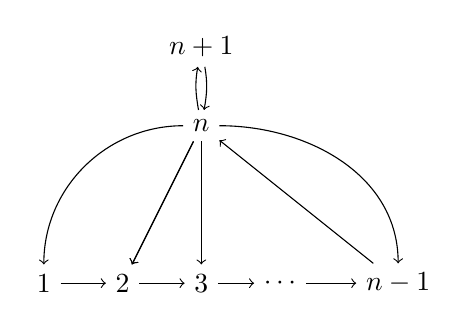
\begin{tikzpicture}
 \node (1) at (1,0) {$1$};
  \node (2) at (2,0) {$2$};
  \node (3) at (3,0) {$3$};
  \node (4) at (4,0) {$\cdots$};
  \node (5) at (5.5,0) {$n -1$};
  \node (n) at (3,2) {$n$};
  \node (nn) at (3,3) {$n + 1$};
\draw[->] (1)--(2);
\draw[->] (2)--(3);
\draw[->] (3)--(4);
\draw[->] (4)--(5);
\draw[->] (n) [out=180, in=90] to (1);
\draw[->] (n)--(2);
\draw[->] (n)--(2);
\draw[->] (n)--(3);
\draw[->] (5)--(n);
\draw[->] (n) [out=0, in=90] to (5);
\draw[->] (n.100) [out=100, in=260] to (nn.260);
\draw[->] (nn.280) [out=280, in=80] to (n.80);
 \end{tikzpicture}
 \]
  Wie beziehen sich die Pageranks (importance scores) zueinander. Sie d"urfen einfach den Pagerank ausrechnen, oder intuitiv erkl"aren welche Seite den h"ohsten Pagerank hat.
  \end{enumerate}
\end{aufgabe}

\end{document}

%%% Local Variables:
%%% mode: latex
%%% End:
